\section{Continuation-Policy Sensitivity (RQ4)}
\label{sec:continuation}

The canonical labels use LRU as the continuation policy after a forced eviction. RQ4 asks whether the optimal-candidate set and regret ordering are materially changed if followed by a different continuation policy. Table~\ref{tab:linkage-continuation-summary} summarizes this sensitivity evidence.

\begin{table}[t]
  \centering
  \footnotesize
  \caption{Offline$\leftrightarrow$closed-loop correspondence and sampled continuation-policy robustness, summarized. Top: H=16 concordance/correlation across the 10 family$\times$capacity cells (\texttt{analysis/closed\_loop\_offline\_linkage\_20260914/}). Bottom: sampled continuation study, Set C (discriminative-under-LRU, $n{=}6597$ primary-sample decisions; \texttt{analysis/continuation\_policy\_sensitivity\_full\_20260914/}), capacities 32/128 only --- population-scale evidence pending census validation.}
  \label{tab:linkage-continuation-summary}
  \begin{tabularx}{\columnwidth}{@{}Lrr@{}}
    \toprule
    \multicolumn{3}{@{}l}{\textit{Offline$\leftrightarrow$closed-loop, H=16 (n=10 cells; SIEVE excluded, no offline counterpart)}} \\
    \midrule
    metric & MRU-vs-LRU & random-vs-LRU \\
    \midrule
    Concordant / discordant / tied (of 10) & 7/1/2 & 6/2/2 \\
    Pearson $r$ & 0.835 & 0.755 \\
    Spearman $\rho$ & 0.915 & 0.829 \\
    Kendall $\tau$-b & 0.773 & 0.591 \\
    \midrule
    \multicolumn{3}{@{}l}{\textit{Sampled continuation robustness, Set C, by capacity}} \\
    \midrule
    metric & cap.\ 32 & cap.\ 128 \\
    \midrule
    MRU median / mean Jaccard & 1.000 / 0.9958 & 1.000 / 0.9999 \\
    MRU mean cross-cont.\ regret & 0.0018 & 0.0001 \\
    MRU strict reversal fraction & 2.7$\times10^{-5}$ & 0.0 \\
    random median / mean Jaccard & 1.000 / 0.7251 & 1.000 / 0.8522 \\
    random mean cross-cont.\ regret & 0.0463 & 0.0197 \\
    random strict reversal fraction & 1.0$\times10^{-3}$ & 1.5$\times10^{-6}$ \\
    \midrule
    \multicolumn{3}{@{}l}{\textit{Sampled continuation robustness, Set C, by horizon (both capacities pooled)}} \\
    \midrule
    metric & H=4 & H=16 \\
    \midrule
    MRU median Jaccard & 1.000 & 1.000 \\
    random median Jaccard & 1.000 & 0.881 \\
    \bottomrule
  \end{tabularx}
\end{table}


\textbf{Sampled MRU/random study.} A pre-registered sampled study evaluates 5{,}500 decisions at capacities 32 and 128. By the pre-registered informative-stratum (Set C) rule, both MRU and mean-random continuation classify ROBUST. MRU is very close to LRU: Set-C mean Jaccard is 0.9958 (cap 32) and 0.9999 (cap 128). Mean-random continuation is more perturbing but still robust: mean Jaccard is 0.7251 (cap 32) and 0.8522 (cap 128). 

\textbf{Full-population MRU census.} The full-population MRU census extends the MRU result to all five families and capacities 32, 64, 128, and 256. Across all 2{,}363{,}286 decision-horizon units, mean optimal-set Jaccard is 0.99941, median Jaccard is 1.0, and 98.69\% of records have exact Jaccard 1. Strict preference reversals are extremely rare ($1.87\times10^{-7}$). 

Because 67.31\% of records are all-tied under both LRU and MRU, the pre-registered decisive stratum is Set C (764{,}282 records). Here, mean Jaccard is 0.99846, median Jaccard is 1.0, and mean cross-continuation regret is 0.000638 misses. Since wiki2018 contributes no Set-C records, this is not inflated by the degenerate negative control.

\textbf{Scope and limitations.} Sensitivity is largest at small capacities and long horizons, but remains small in absolute terms. The worst Set-C cell (alibaba-block/cap32/$H=16$) yields mean Jaccard 0.9804 and median 1.0, satisfying the pre-registered robustness criterion. These results substantiate robustness within the evaluated scope (sampled random at capacities 32/128, and full-population MRU). They do not establish population-scale random-continuation robustness or guarantee that arbitrary deployed policies would preserve the ordering.

\begin{figure}[t]
  \centering
  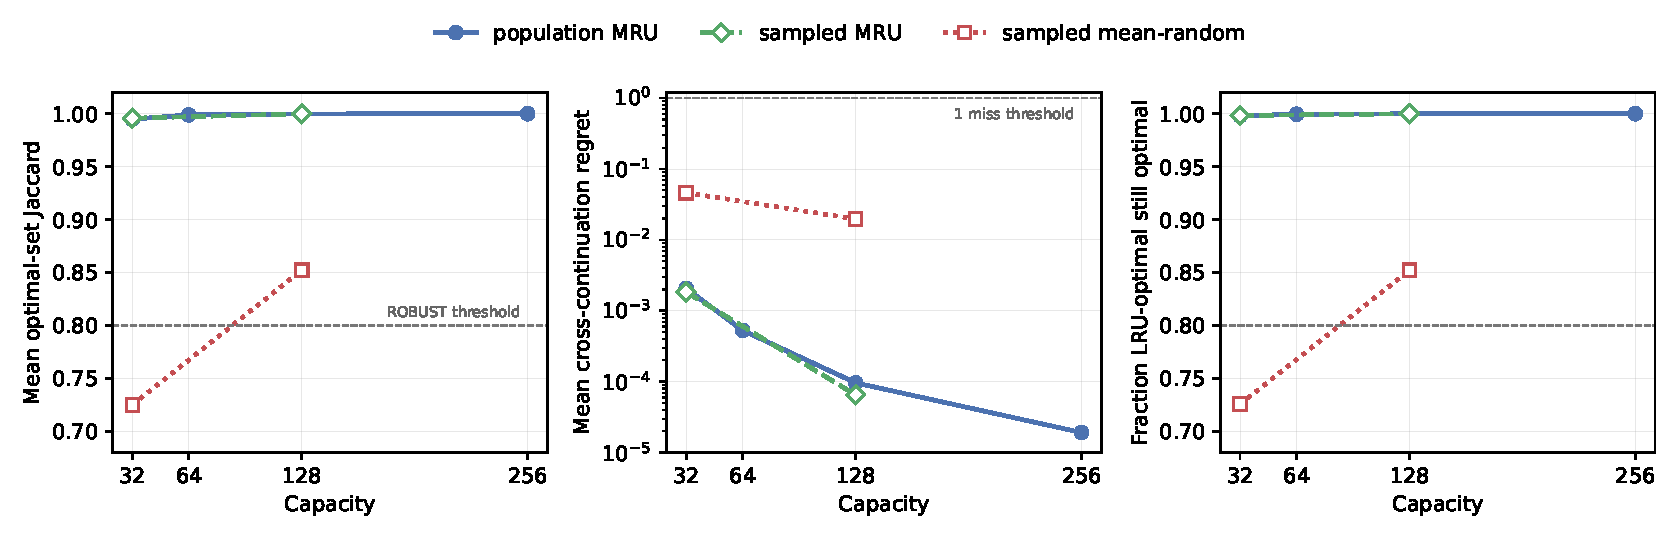
\includegraphics[width=\columnwidth]{figures/figure5_continuation_robustness.pdf}
  \caption{Continuation-policy sensitivity in the pre-registered
  informative stratum (Set C). Sampled MRU and mean-random evidence covers capacities 32 and 128 only;
  full-population MRU evidence covers capacities 32--256.}
  \label{fig:continuation-robustness}
\end{figure}
\FloatBarrier
